\section{N-grams}

\subsection{Implementación}
La implementación de la construcción de los modelos de lenguaje con N-Grams se hizo en el cuaderno de Jupyter: \texttt{HW02\_1}. Esta implementación hizo uso de las siguientes librerías:

\begin{itemize}
    \item \textbf{lxml:} para la lectura de archivos en formato XML.
    \item \textbf{nltk:} para el preprocesamiento del texto.
    \item \textbf{Gensim:} para el \textit{stemming} del texto.
\end{itemize}

En primer lugar fue necesario realizar la lectura de los conjuntos de datos sin procesar y su posterior consolidación en únicos archivos. En el caso del conjunto de datos \textit{20 Newsgroups} se realizó una lectura utilizando la librería estándar de Python. En el caso del conjunto de datos \textit{The Blog Autorship Corpus} fue necesario utilizar la librería \texttt{lxml}. Los dos conjuntos de datos presentaron errores en la codificación, motivo por el cual se asignaron banderas para ignorar y recuperar dichos errores. Los conjuntos de datos consolidados se pueden encontrar en:

\begin{itemize}
    \item \texttt{./resources/news\_consolidate.txt}: consolidado del conjunto de datos \textit{20 Newsgroups}.
    \item \texttt{./resources/blogs\_consolidate.txt}: consolidado del conjunto de datos \textit{The Blog Autorship Corpus}.
\end{itemize}

Una vez consolidados los archivos se procedió al preprocesamiento de los mismos. En primer lugar se realizó una división en oraciones que fueron identificadas con la función \texttt{sent\_tokenize} de \texttt{nltk}. Posteriormente se ejecutaron las siguientes etapas de preprocesamiento sobre cada oración:

\begin{enumerate}
    \item Se convierte el texto a minúscula.
    \item Se reemplazan los números con la palabra \texttt{NUM}.
    \item Se realiza el \textit{stemming} de las palabras de la oración.
    \item Se \textit{tokeniza} la oración teniendo en cuenta los signos de puntuación con el método \texttt{wordpunct\_tokenize} de \texttt{nltk}.
    \item Se eliminan aquellos \textit{tokens} que correspondan a una combinación de signos de puntuación.
    \item Se agregan las etiquetas de inicio y fin de la oración.
\end{enumerate}

Una vez se han procesado todas las oraciones se procede a reemplazar los \textit{tokens} únicos con su etiqueta correspondiente. Este proceso consume la mayor parte del tiempo de ejecución del preprocesamiento debido a la estructura de las listas de Python. Dejando a un lado el reemplazo de los \textit{tokens} únicos, la tabla \ref{tab:ngrams_preproc} presenta algunas estadísticas relevantes al preprocesamiento. Considerando el reemplazo de los \textit{tokens} únicos se tiene que el tiempo de procesamiento es de 1959 y 2112 segundos para \textit{20 Newsgroups} y \textit{The Blog Autorship Corpus} respectivamente.

\begin{table}[h]
    \centering
    \begin{tabular}{|c|c|c|}
        \textbf{Dataset}  & \textbf{20N} & \textbf{BAC} \\
        Tamaño del corpus & 6248453 & 6472811 \\
        Tamaño del vocabulario & 135131 & 107759 \\
        \textit{Tokens} únicos & 70673 & 56323 \\
        \textit{Tokens} finales & 64459 & 51436 \\
        Tiempo de procesamiento & 22.66 s & 25.27 s
    \end{tabular}
    \caption{Estadísticas relevantes para el preprocesamiento de los conjuntos de datos \textit{20 Newsgroups} y \textit{The Blog Autorship Corpus}.}
    \label{tab:ngrams_preproc}
\end{table}

Una vez los conjuntos de datos son procesados, estos son almacenados en dos archivos:

\begin{itemize}
    \item \texttt{./resources/20N\_7\_data.csv}: archivo de valores separados por coma con los \textit{tokens} procesados del conjunto de datos \textit{20 Newsgroups}.
    \item \texttt{./resources/BAC\_7\_data.csv}: archivo de valores separados por coma con los \textit{tokens} procesados del conjunto de datos \textit{The Blog Autorship Corpus}.
\end{itemize}

Tras haber almacenado los datos procesados estos son divididos en dos conjuntos: entrenamiento y validación. La división de los datos se hace utilizando la librería \texttt{scikit-learn}. Al usar esta librería se garantiza una división en donde los datos son mezclados de forma aleatoria. La división entre datos de entrenamiento y validación constituye el último paso antes de la implementación de los N-Grams.

El primer paso de la implementación de los N-Grams consiste en tres funciones auxiliares que retornan el conteo de unigramas, bigramas y trigramas. Estas funciones auxiliares serán utilizadas para la creación de los modelos de lenguaje utilizando el suavizado de Laplace y la interpolación lineal. En términos generales, estas funciones crean un diccionario donde la llave son la o las palabras que componen el N-gram y el valor es el número de veces que estos aparecen en el corpus de entrenamiento. Dentro de la implementación de estas funciones auxiliares no se tienen en cuenta N-grams que no aparezcan en el corpus de los datos de entrenamiento.

Una vez se ha realizado la implementación de estas funciones auxiliares se procede a la implementación de funciones que generen los modelos de lenguaje. Las funciones generadoras de los modelos de lenguaje retornan dos elementos: las probabilidades de los N-grams y un coeficiente estándar para N-grams fuera del vocabulario. La construcción de estos modelos se hace considerando el suavizado de Laplace con $k=1$. El cálculo de la probabilidad para un N-gram se hace como se indica en la ecuación (\ref{eq:n-gram}) donde $V$ es el tamaño del vocabulario. El conteo de los N-grams tanto del mismo orden del que se está calculando como el de los inferiores se obtiene con las funciones auxiliares presentadas previamente.

\begin{equation}
    P(w_{n} | w_{n-1} ) = \frac{count(w_{n-1} w_n ) + 1}{count(w_{n-1}) + V}
    \label{eq:n-gram}
\end{equation}

En base a la implementación de estos N-grams se construye un cuarto modelo que utiliza una interpolación lineal de los mismos. Para ello se definen tres parámetros $\lambda$ que se son optimizados con una estrategia inspirada en el descenso de gradiente estocástico. Con el fin de implementar dicho descenso de gradiente se debe definir una métrica que permita establecer la influencia del cambio de los parámetros. En este caso la métrica a usar corresponde a la perplejidad. Adicionalmente, con el fin de restringir los $\lambda$, los valores son normalizados una vez son calculados. La ecuación \ref{eq:sgd_lamda} presenta el algoritmo de descenso de gradiente, donde $\alpha$ es la tasa de aprendizaje.

\begin{equation}
    \lambda^{i+1} = \lambda^{i} - \alpha \frac{dP}{d\lambda}
    \label{eq:sgd_lamda}
\end{equation}

\subsection{Resultados}
Como se presento en la sección de implementación, la métrica con la cuál se evalúa de forma intrínseca los modelos de lenguaje es la perplejidad. La perplejidad permite identificar el mejor modelo dependiendo del que tenga el menor valor. En este sentido, se asumirá que el mejor modelo es aquel que presente la menor perplejidad. La tabla \ref{tab:perplexity_laplace} presenta los resultados de la perplejidad promedio calculada sobre el conjunto de validación de los dos conjuntos de datos.

\begin{table}[h]
    \centering
    \begin{tabular}{|c|c|c|}
        \textbf{Modelo} & \textbf{20N} & \textbf{BAC} \\
        Unigrama  & 1289 & 806 \\
        Bigrama  & 16230 & 18975 \\
        Trigrama  & 4588633 & 4846085 \\
    \end{tabular}
    \caption{Perplejidad promedio de los tres modelos contemplados sobre los datos de prueba de \textit{20N} y \textit{BAC}.}
    \label{tab:perplexity_laplace}
\end{table}

De los resultados de la tabla \ref{tab:perplexity_laplace} se pueden inferir una serie de consideraciones. En primer lugar, los modelos no cumplen con la condición esperada en la que modelos más complejos tienen una menor perplejidad que modelos más simples. Para los dos conjuntos de datos se tiene que la perplejidad aumenta. En comparación, se tiene que el conjunto de datos del \textit{Wall Street Journal} presenta la progresión de la tabla \ref{tab:perplexity_wsj}, donde la perplejidad disminuye en modelos más complejos. 

\begin{table}[h]
    \centering
    \begin{tabular}{|c|c|c|}
        \textbf{Unigrama} & \textbf{Bigrama} & \textbf{Trigrama} \\
        962 & 170 & 109
    \end{tabular}
    \caption{Progresión de la perplejidad para unigramas, bigramas y trigramas entrenados sobre el conjunto de datos del \textit{Wall Street Journal}.}
    \label{tab:perplexity_wsj}
\end{table}

En este caso, vale la pena revisar la relación entre el número de \textit{tokens} en la colección y el tamaño del vocabulario. En el caso de \textit{20N} se tiene un tamaño de la colección de 6248453 \textit{tokens} y un vocabulario de 64459 \textit{tokens}, una vez se han eliminado los \textit{tokens} únicos. Para el conjunto de datos \textit{20N} se tiene que la relación entre el tamaño del corpus y el vocabulario es de 96.94. De forma similar, para el caso del conjunto de datos \textit{BAC} la relación es de 125 y para el conjunto de datos del \textit{WSJ} es de 1901. 

La relación entre el tamaño del corpus y del vocabulario permite asumir que el número de repeticiones de un N-gram es menor para los conjuntos de datos de \textit{20N} y \textit{BAC} en comparación al \textit{WSJ}. En este sentido, se tiene que el cálculo de la perplejidad va a utilizar el coeficiente estándar en vez de las probabilidades calculadas. Esta situación se debe a que al tener un vocabulario tan extenso, es más frecuente que aparezcan términos no considerados en el vocabulario inicial en el conjunto de validación. Esta situación se evidencia al comparar la perplejidad para varias oraciones y notar como el valor que toma es similar. 

La figura \ref{fig:perplexity_sentences} presenta valores de perplejidad para tres modelos de lenguaje distintos: unigramas, bigramas y trigramas. Note como los valores de perplejidad para el modelo de trigramas son similares entre las distintas oraciones. Esto indica que los valores de probabilidad usados para calcular la perplejidad también son similares entre ellos. La manera en la cual se puede presentar esta situación es que se utilice el coeficiente por defecto del modelo, lo cual a su vez demuestra que los trigramas considerados en el conjunto de validación no estaban presentes, en su mayoría, en el modelo.

\begin{figure}[h]
    \centering
    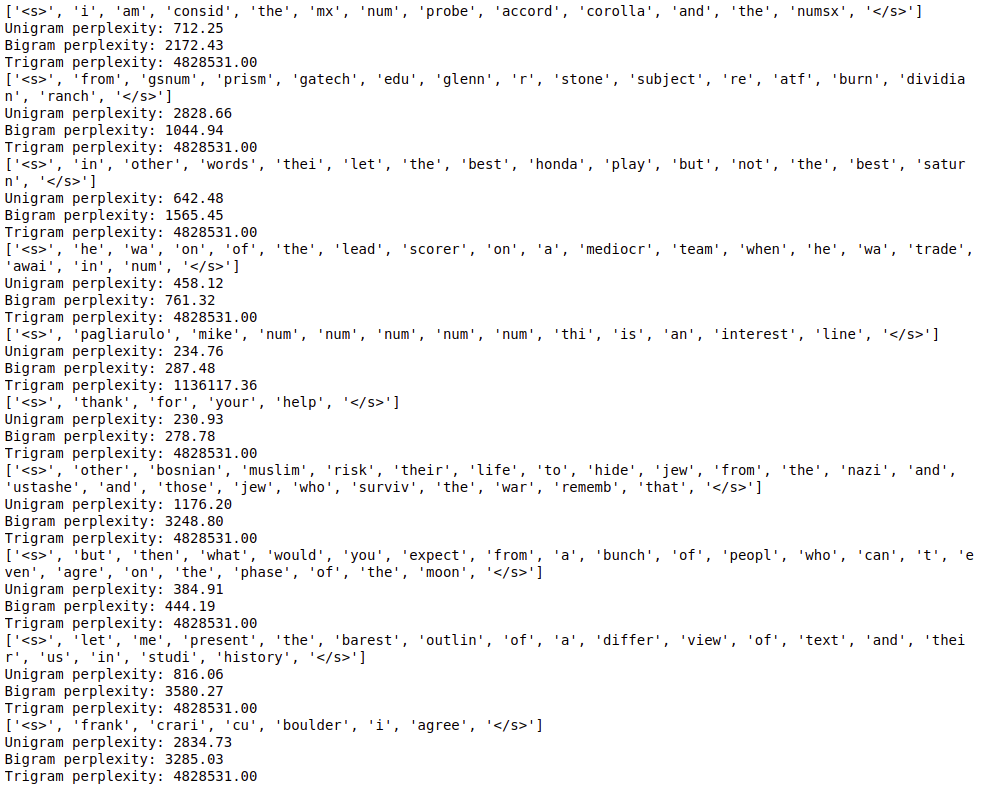
\includegraphics[width=\textwidth]{doc/images/perplexity.png}
    \caption{Cálculo de la perplejidad para distintas oraciones con diferentes modelos de lenguaje.}
    \label{fig:perplexity_sentences}
\end{figure}

Existen dos alternativas para solucionar esta situación y mejorar la calidad de los modelos de lenguaje: aumentar el tamaño del corpus ó disminuir el tamaño del vocabulario. Dado que aumentar el tamaño del corpus no es viable dada la antigüedad de los conjuntos de datos, se debería proceder a disminuir el vocabulario de los mismos. Un factor a tener en cuenta es que debido a los requerimientos del enunciado, no se eliminaron las palabras de parada (\textit{stopwords}). Una opción viable para este caso sería eliminar las palabras de parada, con lo cual se reduciría el tamaño del vocabulario. Otra alternativa sería la incorporación de más etapas de preprocesamiento de los datos con el fin de reducir el tamaño del vocabulario.

